% !TEX encoding = UTF-8 Unicode
\documentclass{article}

\usepackage{fontspec}   %加這個就可以設定字體
\usepackage{xeCJK}       %讓中英文字體分開設置
\setCJKmainfont{BiauKai} %設定中文為系統上的字型,而英文不去更動,使用原TeX字型
\setmainfont{Times} % 設定英文字型
\XeTeXlinebreaklocale "zh"             %這兩行一定要加,中文才能自動換行
\XeTeXlinebreakskip = 0pt plus 1pt     %這兩行一定要加,中文才能自動換行

\usepackage{titling}
\setlength{\droptitle}{-12em} % 將標題移動至頁面的上面


\title{第一章 - 準備好你的鴨子車!}

\author{呂承龍}
\date{} %不要日期

\begin{document}
\maketitle

\section{鴨子車硬體設備介紹}
\subsection{鴨子車}
鴨子車是我們在鴨子城裡主要的機器人,我們會利用他做自動道路駕駛以及各式各樣的實驗。首先我們先介紹鴨子車的硬體架構。
\\
\begin{figure}[htp]
    \begin{center}
        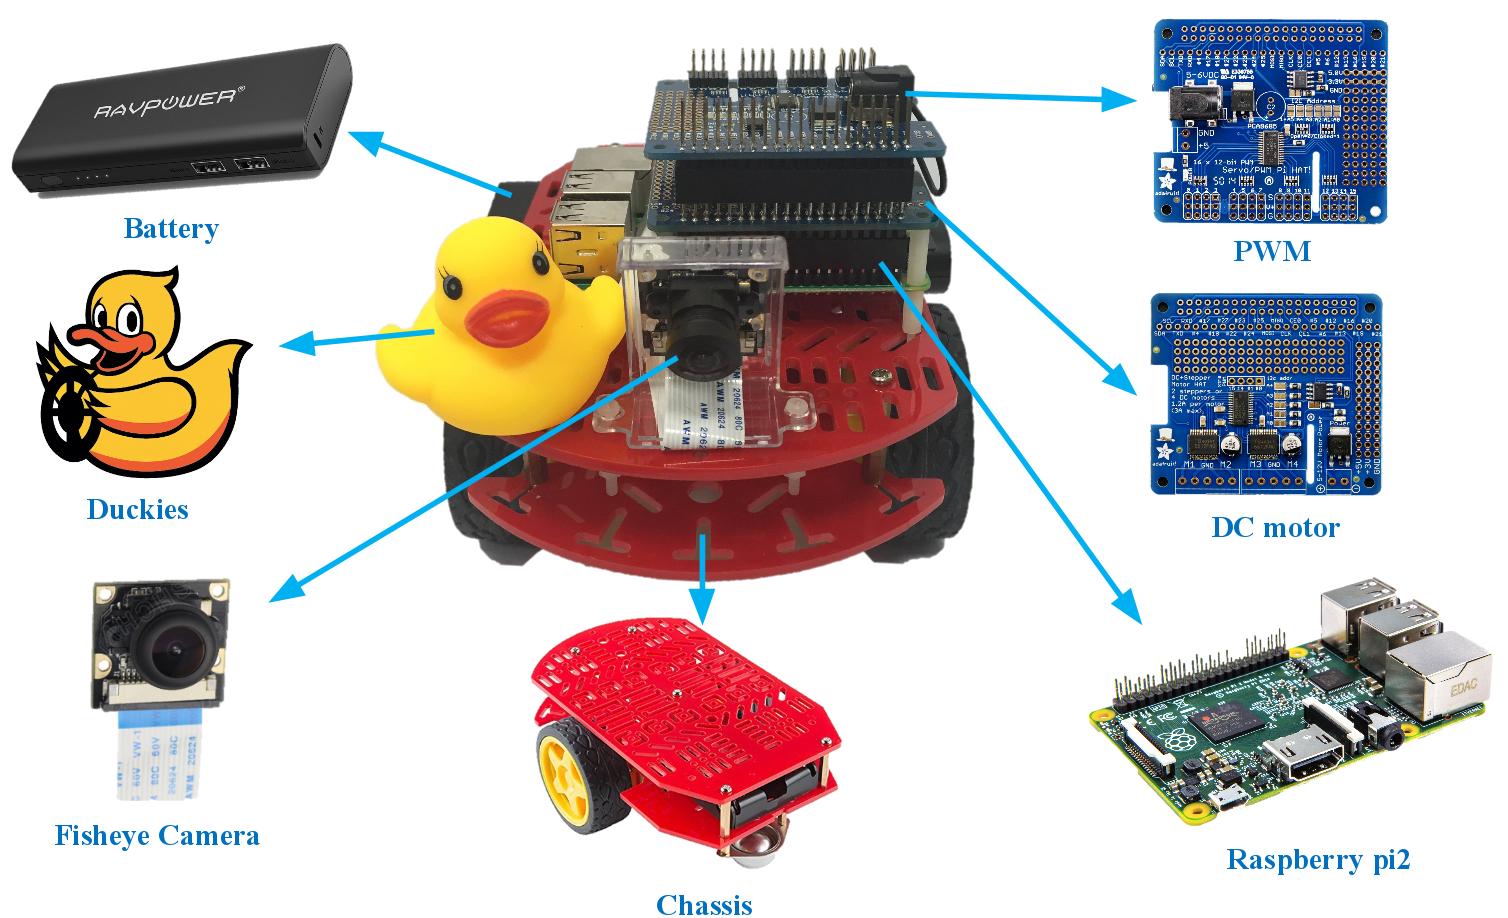
\includegraphics[width=250pt]{pic/1_1_1.png}
    \end{center}
\end{figure}

\subsection{車殼}
你可以在Amazon買到這台車的車殼,英文名字Amazon Magician Chassis,模組編號:SX10825
\\購買網址:https://goo.gl/L6opq3
\\
\begin{figure}[htp]
    \begin{center}
        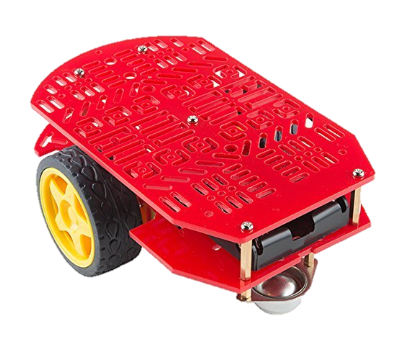
\includegraphics[width=150pt]{pic/1_1_23.png}
    \end{center}
\end{figure}

\subsection{樹莓派2 Model B}
樹莓派是一塊嵌入式板子,你可以把它看作是一台小電腦,上面一樣有中央處理器、記憶體等等。我們會在上面運行Linux Ubuntu14.04的作業系統。
\\購買網址:https://goo.gl/iYWy1p
\\
\begin{figure}[htp]
    \begin{center}
        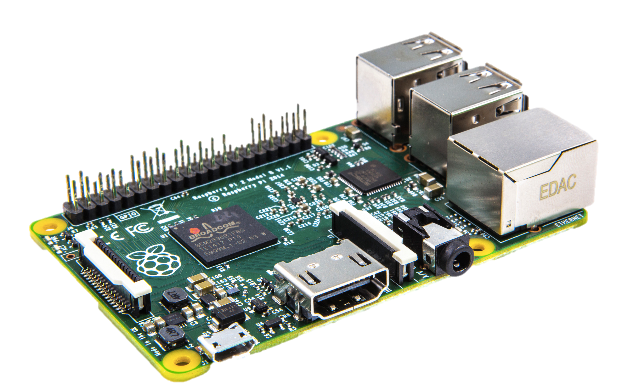
\includegraphics[width=150pt]{pic/1_1_2.png}
    \end{center}
\end{figure}

\subsection{搖桿接收器、無線網卡、隨身碟}
接下來由左而右分別是搖桿接收器、無線網卡、隨身碟。搖桿可以拿來控制車子,我們使用的是羅技的F710。而無線網卡是為要讓電腦與車子特過Wifi進行連線,我們使用ASUS USB-N10 Nano。隨身碟則是可以儲存log data時的資料,這裡只需準備32G隨身碟即可。
\\
\begin{figure}[htp]
    \begin{center}
        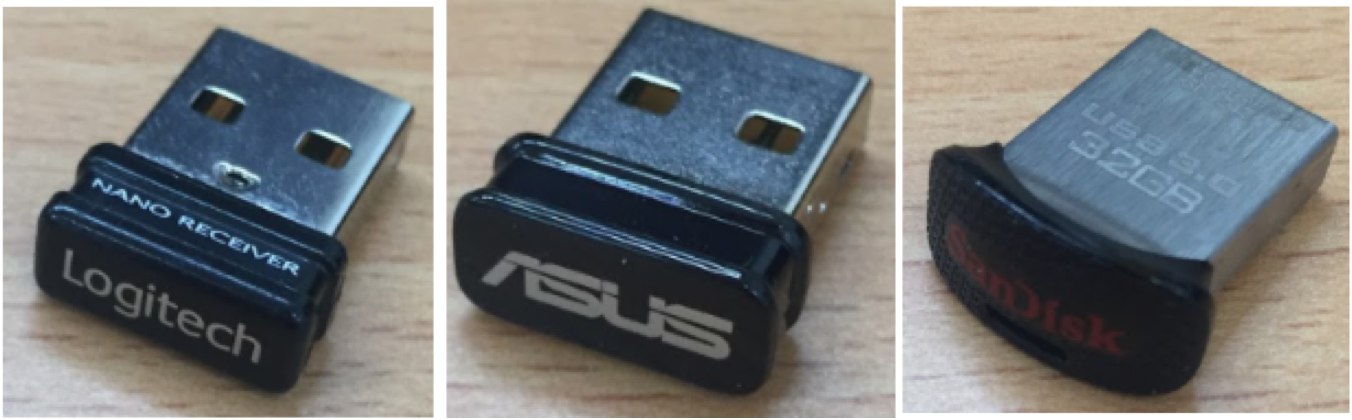
\includegraphics[width=250pt]{pic/1_1_3.png}
    \end{center}
\end{figure}
\\\\
\subsection{RPi 鏡頭 (G)}
這款鏡頭可以支援所有版本的樹莓派,視角寬度達160度,最高解析度達1080p。
\\購買網址:https://goo.gl/z1ozEU
\\
\begin{figure}[htp]
    \begin{center}
        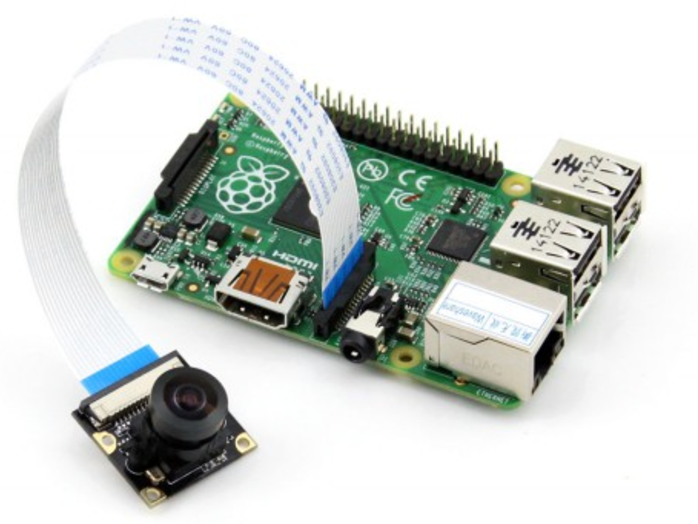
\includegraphics[width=250pt]{pic/1_1_4.png}
    \end{center}
\end{figure}

\subsection{PWM板及馬達驅動板}
PWM板的目的是要用PWM的技術控制馬達驅動。PWM 是一種利用數位訊號模擬類比訊號的方式去控制馬達轉速的技術。我們使用的是Adafruit 16-Channel
PWM / Servo HAT (左為PWM板/右為馬達驅動板)
\\購買網址:https://goo.gl/jrC2dL
\\
\begin{figure}[htp]
    \begin{center}
        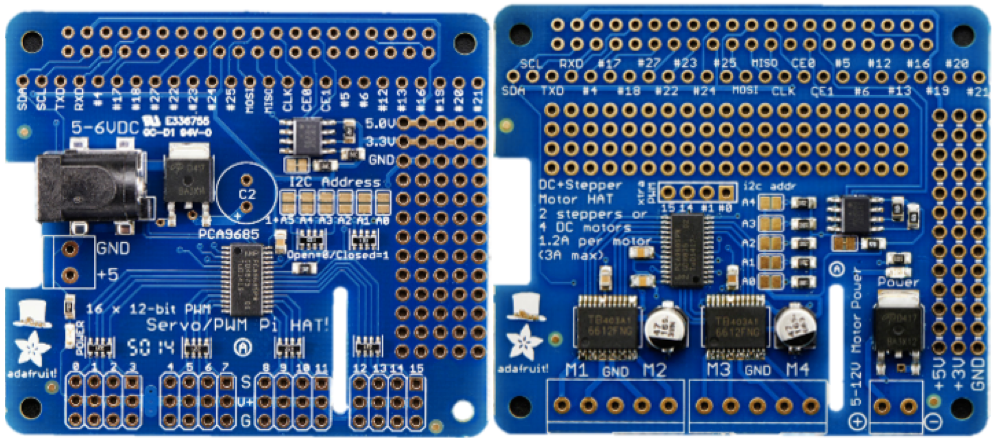
\includegraphics[width=250pt]{pic/1_1_5.png}
    \end{center}
\end{figure}

\subsection{行動電源}
另外需要購買一個有兩個USB輸出的行動電源,以及一個USB轉DC的轉接頭。這部分買自己喜歡的就可以了!

\subsection{焊接}
最後我們要講解如何焊接。
\\首先,我們要先焊馬達驅動板,請不要拿錯。將2 pin和3 pin的電子零件卡在一起(旁邊有卡榫處)
\\
\begin{figure}[htp]
    \begin{center}
        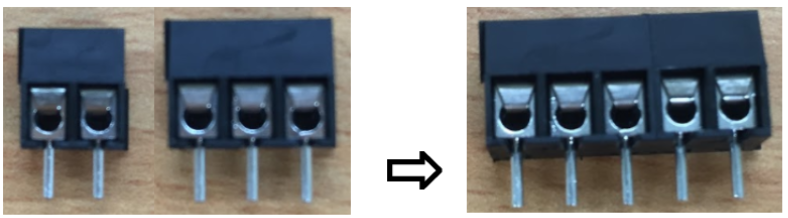
\includegraphics[width=250pt]{pic/1_1_6.png}
    \end{center}
\end{figure}
\\
將做完的5 pin電子零件焊接到馬達驅動板上對應的Pin角 "M1 GND M2" (M1與M2之後都會接到馬達上,M3與M4此課程毋須用到) (不要焊錯方向)
\\
\begin{figure}[htp]
    \begin{center}
        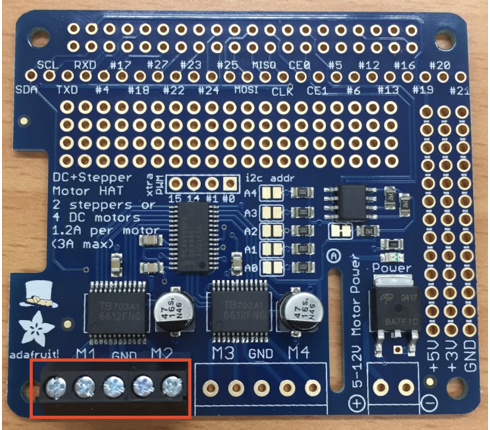
\includegraphics[width=150pt]{pic/1_1_7.png}
    \end{center}
\end{figure}
\\
將此 2 pin 的電子零件焊接到馬達驅動板的Pin角”power” (不要焊錯方向)
\\
\begin{figure}[htp]
    \begin{center}
        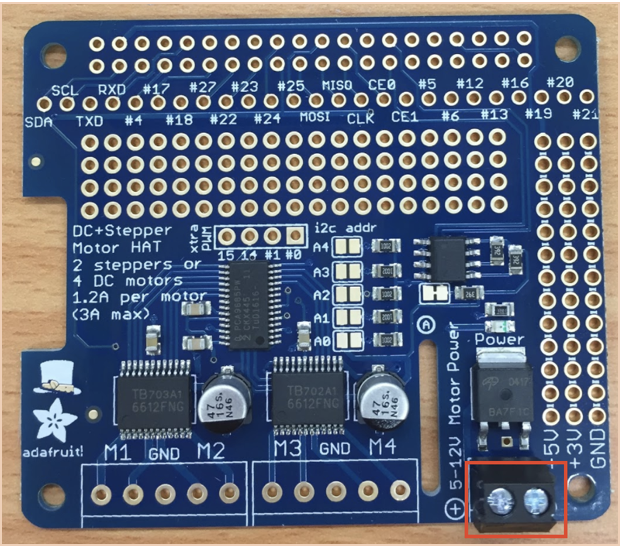
\includegraphics[width=150pt]{pic/1_1_8.png}
    \end{center}
\end{figure}
\\
將排針組(此電子零件有2x20個接角)以右圖方式焊到電路板(不要焊錯方向)
\\
\begin{figure}[htp]
    \begin{center}
        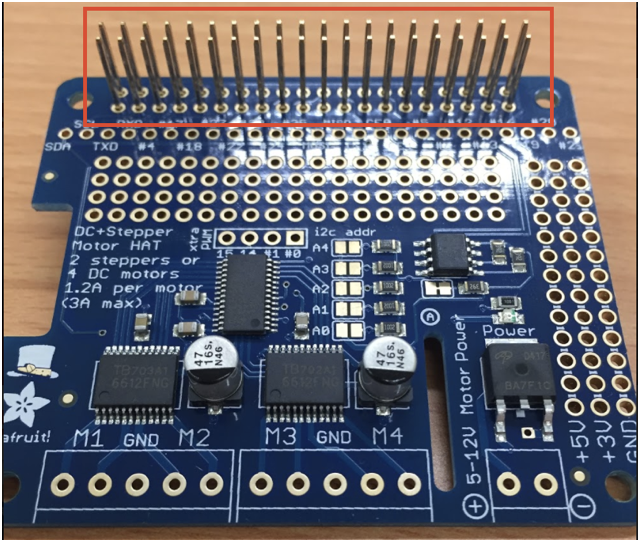
\includegraphics[width=150pt]{pic/1_1_24.png}
    \end{center}
\end{figure}
\\
再來要焊PWM板。 將此2 pin的電子零件以圖片方式焊到PWM板上(在電源孔旁邊)(不要焊錯方向) 
\\
\begin{figure}[htp]
    \begin{center}
        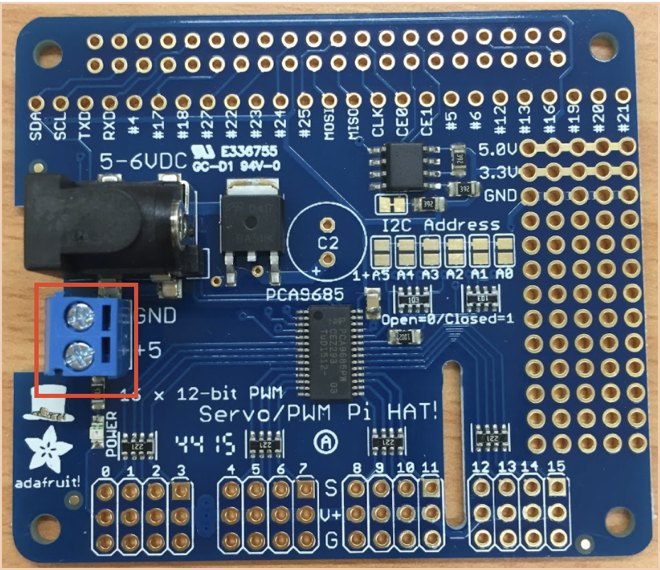
\includegraphics[width=150pt]{pic/1_1_9.png}
    \end{center}
\end{figure}
\\
將排針組(此電子零件有2x20個接角)以圖片方式焊到PWM板上(不要焊錯方向)
\\
\begin{figure}[htp]
    \begin{center}
        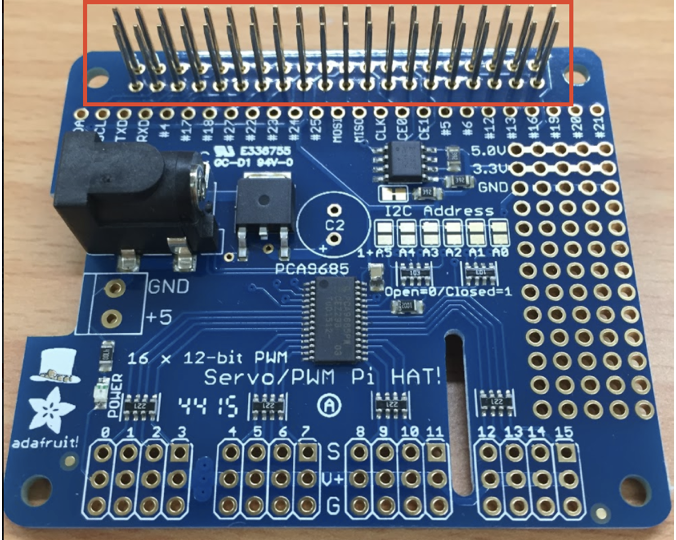
\includegraphics[width=110pt]{pic/1_1_10.png}
    \end{center}
\end{figure}
\\
將此 3x4孔針頭的排針組以下圖方式焊到PWM板上標籤 "Servo/PWM Pi HAT!"的位置(不要焊錯方向)
\\
\begin{figure}[htp]
    \begin{center}
        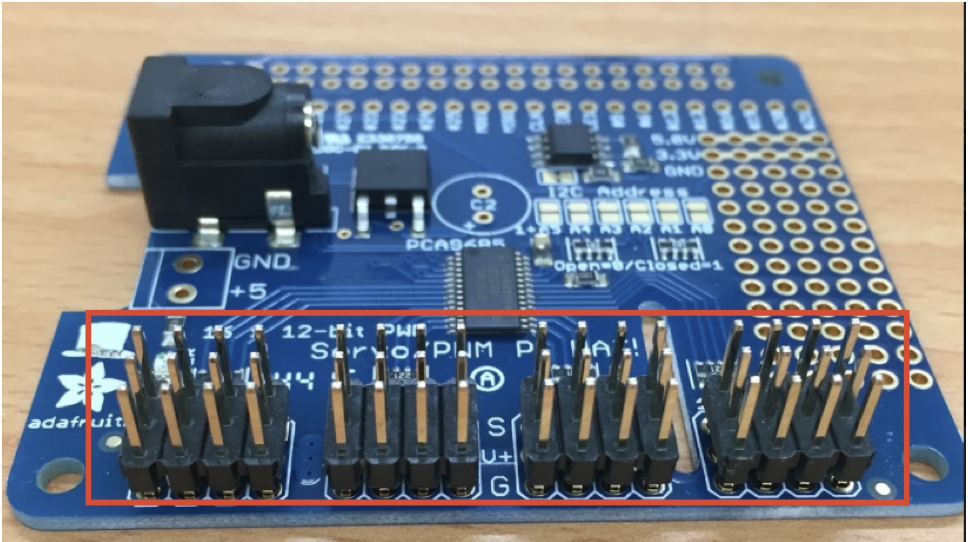
\includegraphics[width=150pt]{pic/1_1_11.png}
    \end{center}
\end{figure}

\subsection{車體組裝}
首先一定要檢查零件,其中我們不需要用到電池盒的部分。
\\
\begin{figure}[htp]
    \begin{center}
        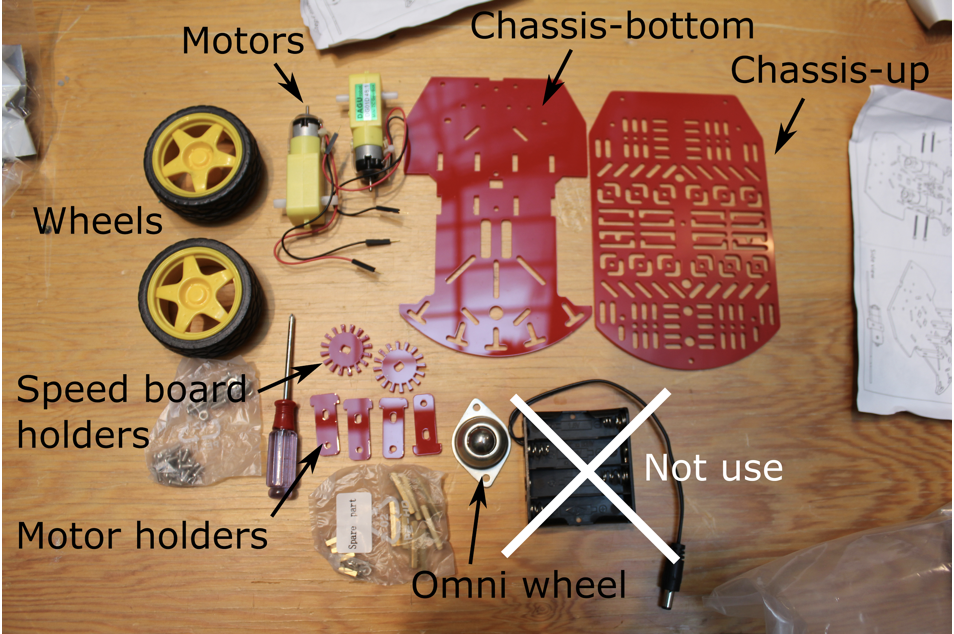
\includegraphics[width=150pt]{pic/1_1_12.png}
    \end{center}
\end{figure}
\\
先將馬達固定框裝到車殼上,編碼器齒輪裝在馬達靠近車體內側,將此編碼器齒輪裝在馬達靠近車體內側後,用螺絲把馬達鎖到車殼上(使用最長的3mm螺絲與3mm的螺帽)
\\
\begin{figure}[htp]
    \begin{center}
        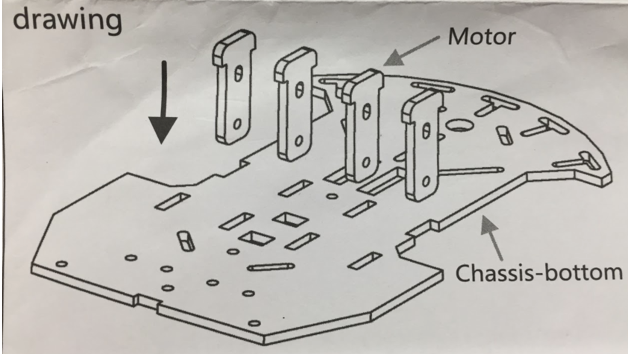
\includegraphics[width=150pt]{pic/1_1_13.png}
    \end{center}
\end{figure}
\\
\\
\begin{figure}[htp]
    \begin{center}
        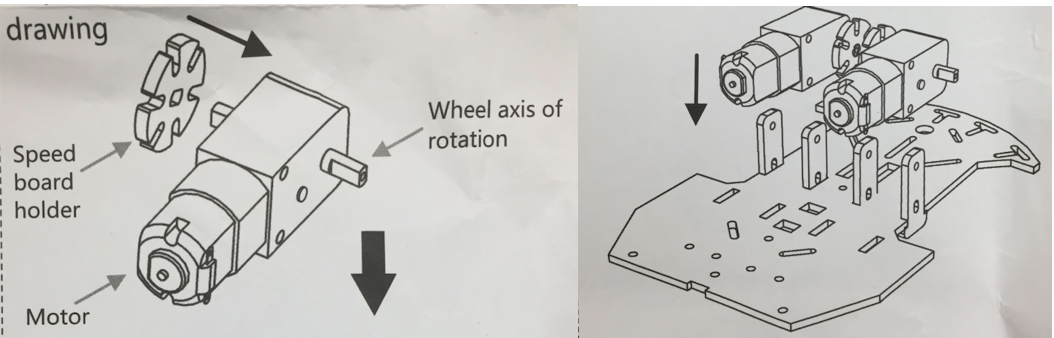
\includegraphics[width=300pt]{pic/1_1_14.png}
    \end{center}
\end{figure}
\\
\\
\begin{figure}[htp]
    \begin{center}
        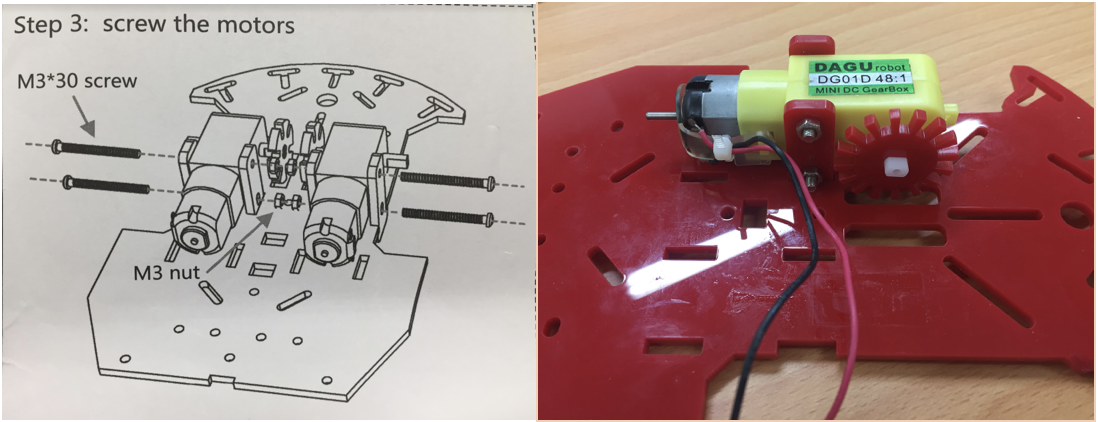
\includegraphics[width=300pt]{pic/1_1_15.png}
    \end{center}
\end{figure}
\\
將輪胎裝到車子底盤上
\\
\begin{figure}[htp]
    \begin{center}
        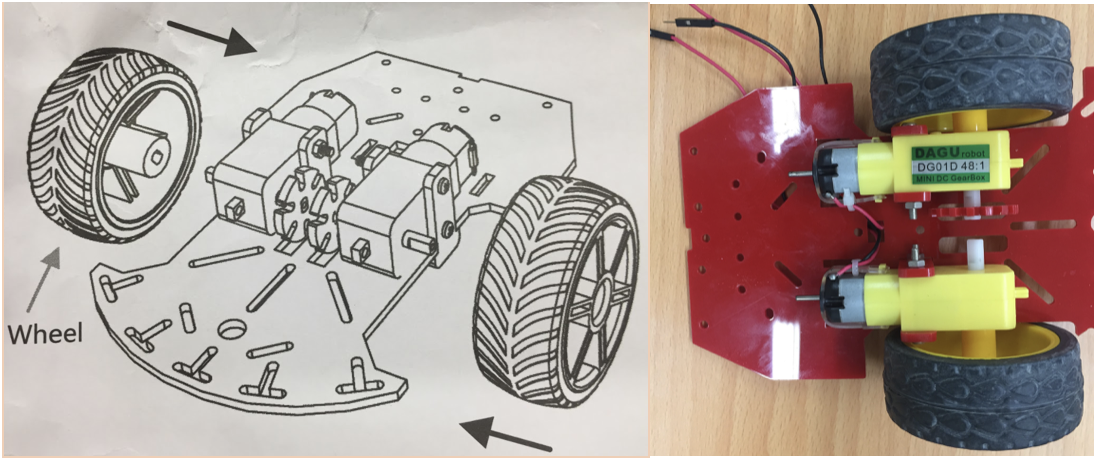
\includegraphics[width=300pt]{pic/1_1_16.png}
    \end{center}
\end{figure}
\\
將萬向輪裝到車子底盤上
\\
\begin{figure}[htp]
    \begin{center}
        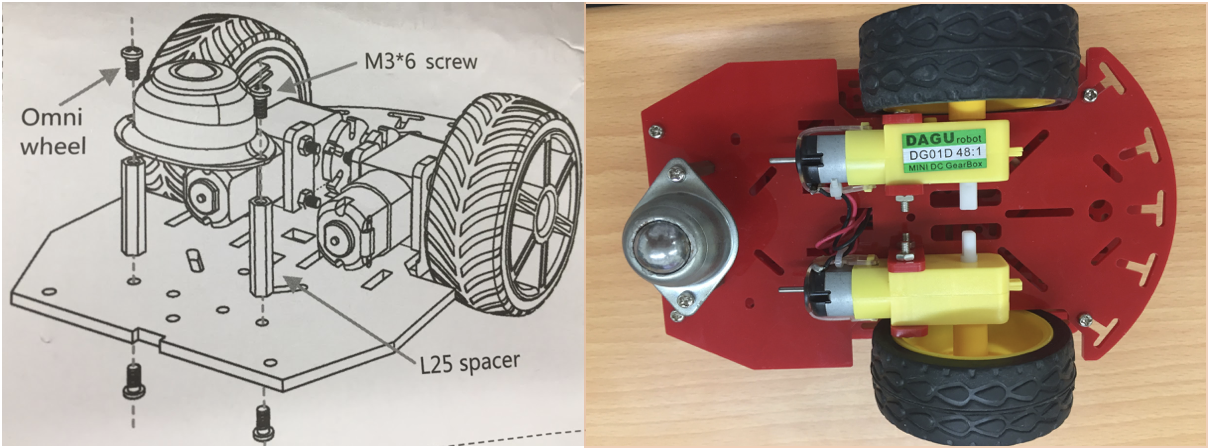
\includegraphics[width=300pt]{pic/1_1_17.png}
    \end{center}
\end{figure}
\\
\\\\\\\\\\\\\\將銅柱鎖到車子底盤上
\\
\begin{figure}[htp]
    \begin{center}
        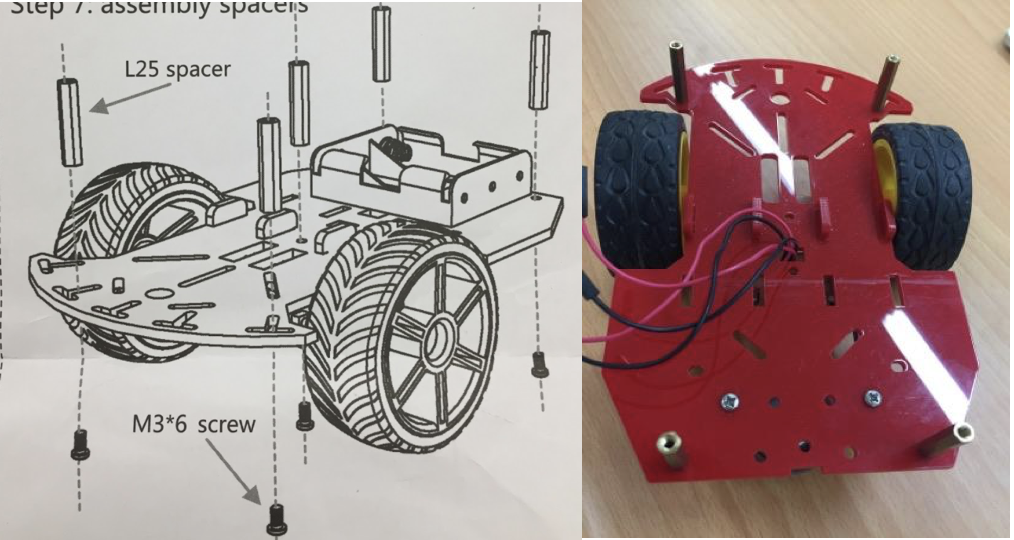
\includegraphics[width=250pt]{pic/1_1_18.png}
    \end{center}
\end{figure}
\\
現在我們將車子底盤部分完成了! 先別急著把另一片車板裝上去.
\\我們要先來將pi裝上去,用8個塑膠支架把樹莓派裝在上車版,並用塑膠螺帽將它固定
\\
\begin{figure}[htp]
    \begin{center}
        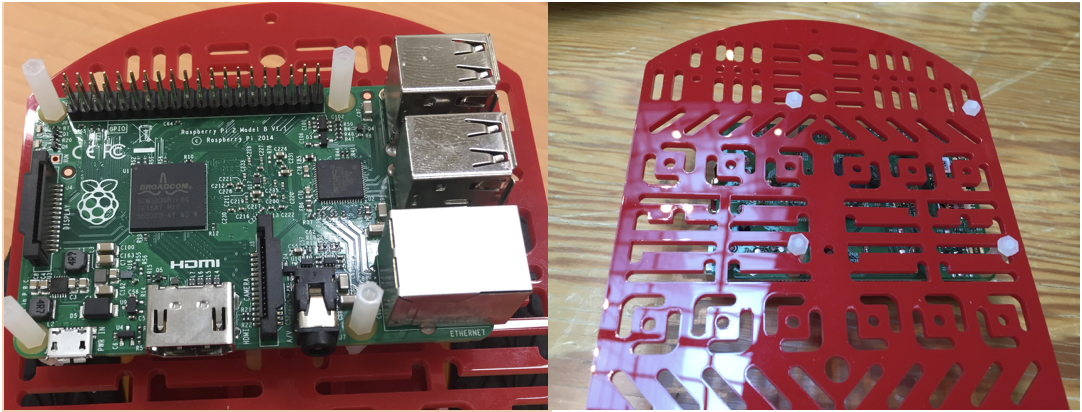
\includegraphics[width=250pt]{pic/1_1_19.png}
    \end{center}
\end{figure}
\\
將塑膠螺絲把鏡頭框架與鏡頭裝在上車板,並將鏡頭與樹莓派用線接在一起連接方式: 觀察樹莓派與鏡頭上的電線連接處,我們可以將其卡榫拉開,並將線插進去(注意方向,不然鏡頭會燒掉),之後再鎖上卡榫便可完成。鏡頭架可在這裡購買:https://goo.gl/6TyaYN
\\
\begin{figure}[htp]
    \begin{center}
        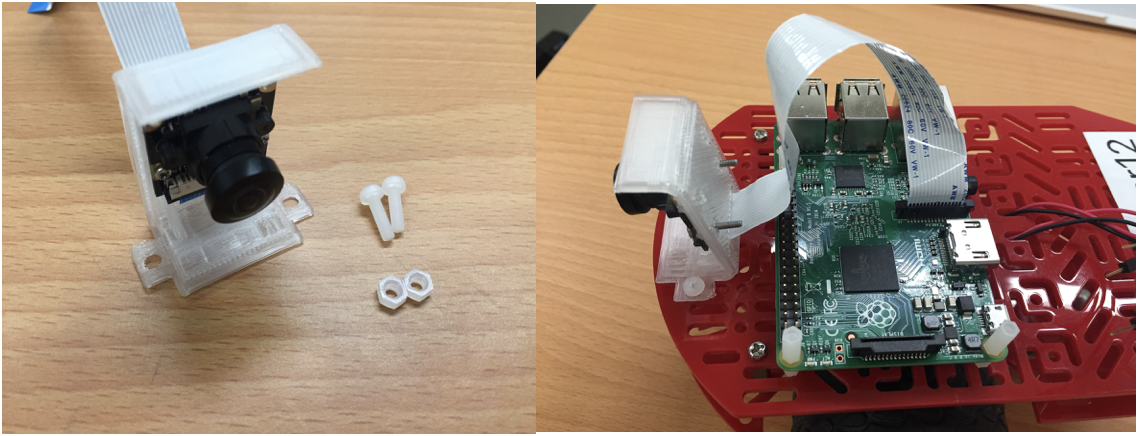
\includegraphics[width=250pt]{pic/1_1_20.png}
    \end{center}
\end{figure}
\\
將電路板DC+Stepper Motor Hat 用塑膠支架裝在樹莓派上
用杜邦母頭連結馬達與馬達驅動板。我們使用馬達驅動板上的M1與M2來驅動馬達,因此左邊的馬達連結兩條線到M1的兩個pin角,右邊的馬達連結兩條線到M2的兩個pin角。
\\
\begin{figure}[htp]
    \begin{center}
        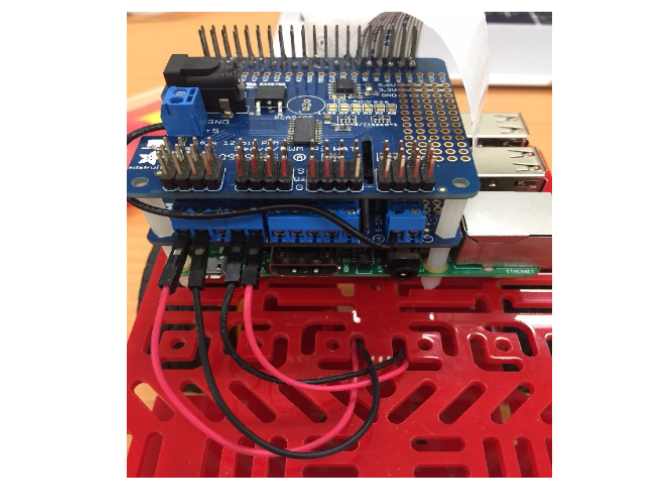
\includegraphics[width=200pt]{pic/1_1_21.png}
    \end{center}
\end{figure}
\\
將行動電源放到車板中間,接著再將充電線連接到行動電源與樹莓派、USB轉DC接到行動電源與馬達驅動板。就完成囉!

\newpage
\section{鴨子車作業系統準備}
\subsection{作業系統}
要使用RPi這種板子一定要作業系統。鴨子車上的作業系統也是Ubuntu 14.04,這部分請準備一張32GB的SD卡,並視情況準備一個給SD卡用的USB Adapter。接下來我們要將鴨子車上的作業系統燒進SD卡。同時也會教大家,如果我們要把此時的作業系統存進電腦裡該怎麼做。

\subsection{作業系統燒錄}
先下載Win32DiskImager:https://goo.gl/GWEKRJ
\\將SD卡格式化之後,插進電腦裡,選擇作業系統映像檔的位址。再按下資料到裝置。
\subsection{作業系統儲存}
將SD卡插進電腦裡,選擇作業系統映像檔要儲存的位址。再按下讀取。
\\
\begin{figure}[htp]
    \begin{center}
        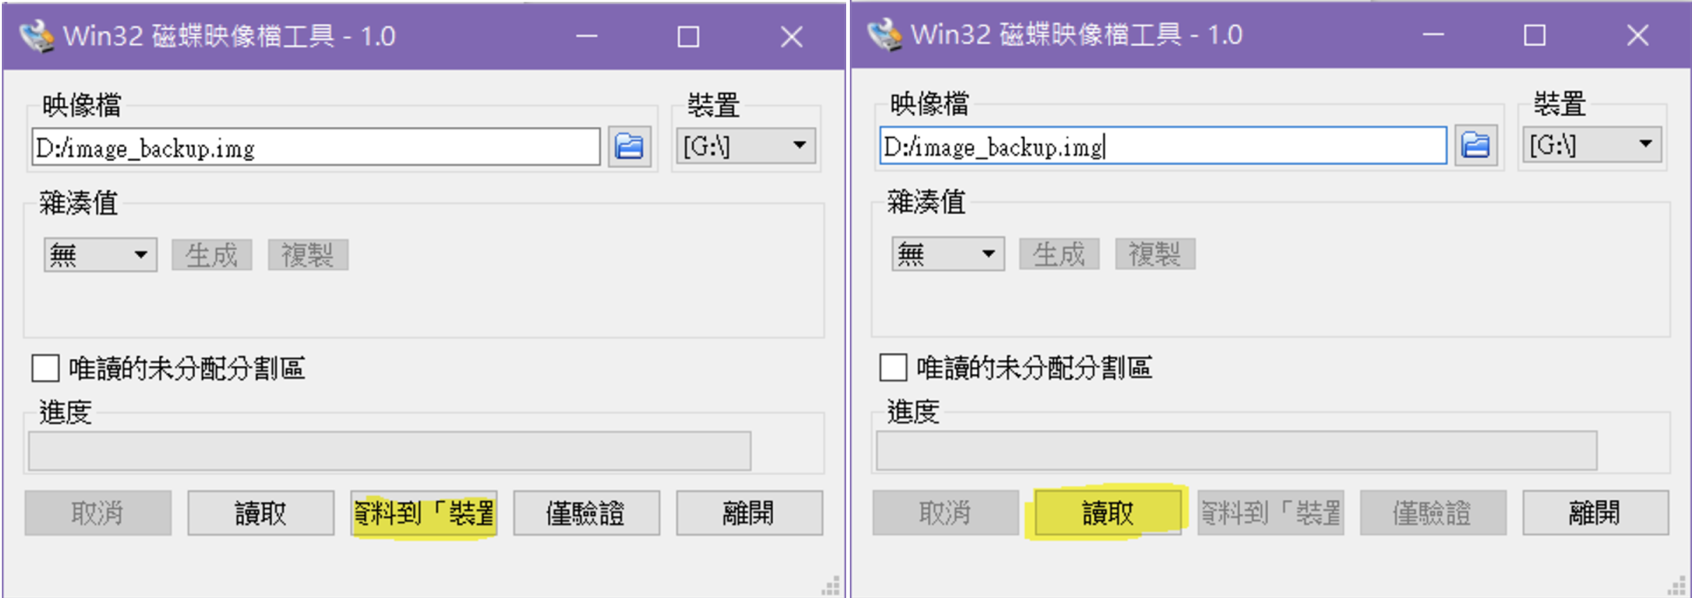
\includegraphics[width=400pt]{pic/1_2.png}
    \end{center}
\end{figure}
\\

\newpage
\section{為鴨子車取名字}
\subsection{想個獨特的名字吧!}
每台鴨子車都應該要有自己獨特的名字,除了軟體需求以外,更是能代表自己特別之處。你可以想像如果車子是你的孩子,或是來紀念一個特別的事物,都是非常有趣的!

\subsection{更改名字}
接下來我們要更改鴨子車的名字了,這裡請準備螢幕(需要HDMI接頭、若只有VGA接頭可去購買轉接頭),以及鍵盤,接上樹莓派之後,請將板子接上電源。等待一會之後,輸入帳號密碼,皆為ubuntu (輸入密碼時不會顯示出來)。就會看到這個畫面
\\
\begin{figure}[htp]
    \begin{center}
        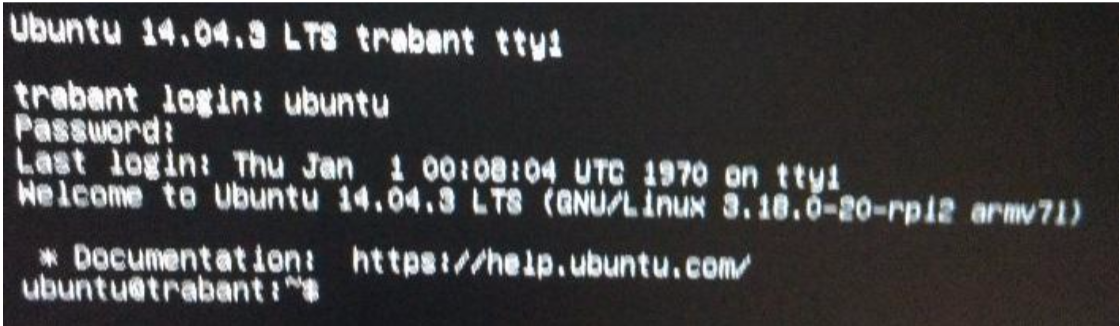
\includegraphics[width=300pt]{pic/1_3_1.png}
    \end{center}
\end{figure}
\\
請輸入 sudo vim /etc/hostname
\\將 “duckiebot” 換成 “你車子的名字” (in this case “test”),請不要使用duckiebot作為車子名稱,第一字不要大寫或數字與標點符號,名字不要有標點符號與大寫。若不會vim的同學,請看書末的appendix。
\\
\begin{figure}[htp]
    \begin{center}
        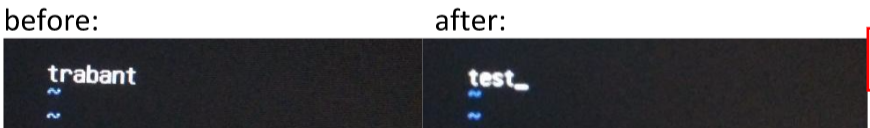
\includegraphics[width=300pt]{pic/1_3_2.png}
    \end{center}
\end{figure}
\\
請輸入 sudo vim /etc/hosts
\\將 “duckiebot” 換成 “你車子的名字” (這個例子是 “test”)
\\
\begin{figure}[htp]
    \begin{center}
        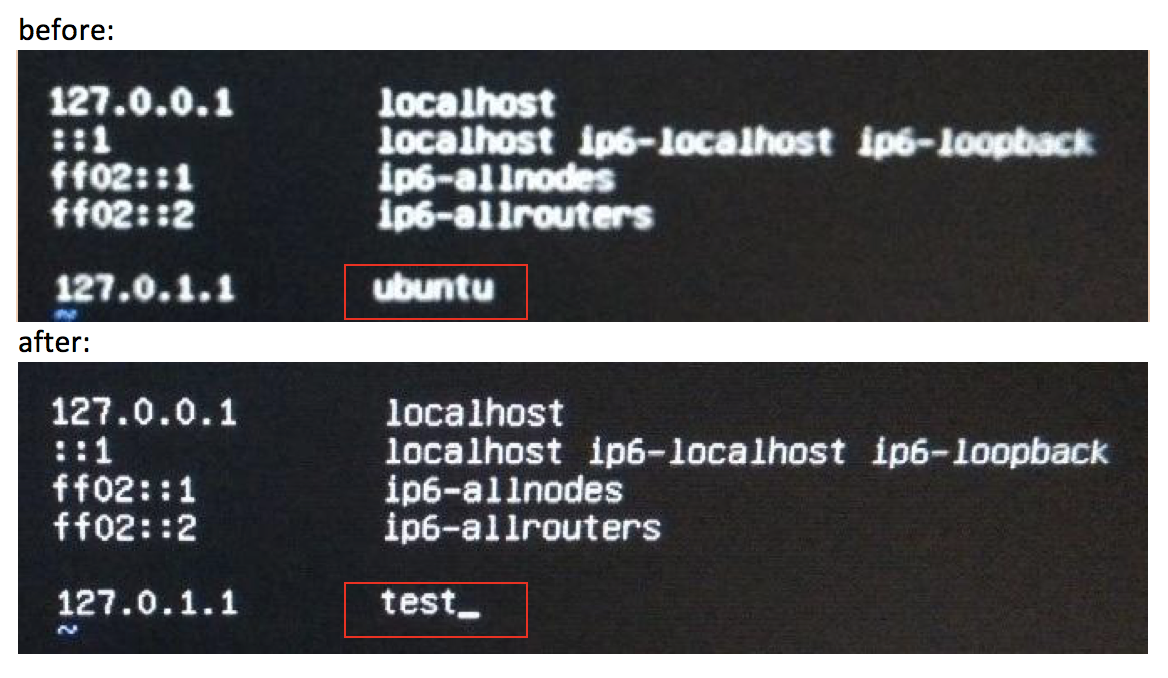
\includegraphics[width=300pt]{pic/1_3_3.png}
    \end{center}
\end{figure}
\\
\\\\\\\\\\\\重新開機,輸入sudo reboot -n。
\\重開機後,你會發現使用者名稱已換成你剛剛設定的車子的名字

\newpage
\section{測試鴨子車}
\subsection{測試相機}
首先先來測試相機,請輸入以下指令。第一個指令會把鏡頭拍到的圖片顯示出來維持10秒鐘,然後存檔。第二個指令可以看到這個資料夾下有什麼檔案,當然就會有剛剛的儲存的檔案。
\\duckiebot \$ raspistill -t 10000 -o out.jpg
\\duckiebot \$ ls

\subsection{測試搖桿}
請依照順序輸入以下指令,第二個指令將會初始化環境,第三個指令將會設定你的鴨子車為ros master),第三個指令將啟動程式,啟動Joystick,接著你可以嘗試使用搖桿來操控車子,按下Logitech按鈕後可以操控車子前後左右。請記得都要將duckiebot改成你的車子的名字。
\\duckiebot \$ cd ~/duckietown
\\duckiebot \$ source environment.sh
\\duckiebot \$ source set\_ros\_master.sh [duckiebot]
\\duckiebot \$ roslaunch duckietown\_demos joystick.launch veh:=[duckiebot]


\end{document}























